\documentclass[11pt]{article}
\usepackage[paper=a4paper,top=1.5cm,left=1.5cm,right=1.5cm,
    foot=1cm,bottom=1.5cm]{geometry}

\usepackage{times}
\usepackage[T1]{fontenc}
\usepackage[utf8]{inputenc}
\usepackage[english,russian]{babel}
\usepackage{amssymb,amsfonts,amsmath,mathtext,amsbsy}
\usepackage{multirow}
\usepackage{listings}
\usepackage{graphicx}
\graphicspath{{./images/}}

\newcommand{\comment}[1]{}
\newcommand{\br}[1]{\boldsymbol{\mathrm{#1}}}
\DeclareMathOperator{\rot}{rot}
\newcommand{\Reyn}{\text{Re}}
\newcommand{\Pran}{\text{Pr}}
\newcommand{\Nuss}{\text{Nu}}

%\newcommand{\br}[1]{\bm{\mathrm{#1}}}

\newenvironment{packed_enum}{
\begin{enumerate}
  \setlength{\itemsep}{1pt}
  \setlength{\parskip}{0pt}
  \setlength{\parsep}{0pt}
}{\end{enumerate}}

\title{VVHD}
\author{Я. А. Дынников}

\begin{document}

\maketitle

%%%%%%%%%%%%%%%%%%%%%%%%%%%%%%%%%%%%%%%%%%%%%%%%%%%%%%%%%%%%%%%%%%%%%%%%%%%%%%%%
\begin{abstract}
Это мануал, посвященный исходникам библиотеки. Здесь я постараюсь 
описать его структуру, способы работы с ним, и подводные камни, 
на которые нужно будет обращать внимание.
\end{abstract}

\section{TList}
Лист является шаблонным классом и надстройкой над массивом. 
Лист предоставляет функции добавления, удаления элементов и 
динамического изменения размеров. В принципе, лист является 
усовершенствованным вектором (из std::), он даже почти полностью
с ним совместим.

\lstset{language=C++, frame=single}
\begin{lstlisting}
template <class T>
class list
{
	public:
		list();
		~list();

		void push_back(const T &item);
		void erase(T* item);
		void clear();
		T& at(size_t i);
		T* begin();
		T* end();
		size_t size();
		size_t size_safe();
		T* next(T* item);
		T* prev(T* item);

	private:
		size_t size_;
		size_t maxsize;
		T* begin_;
		T* end_;

		void realloc_();
};

#define const_for(list, it) \
	for (auto it=list->begin(); it<list->end(); it++)
\end{lstlisting}

Вот о чем нужно помнить
\begin{enumerate}
\item Если вы добавляете в массив элементы, не пользуйтесь 
инкрементом TObj* obj++. Если вдруг произойдет realloc ---
адресация массива сменится непредсказуемо.
\item При удалении элемента на его место перемещается последний 
элемент, а size уменьшается.
Если Вы удалили элемент функцией erase(), не забудте указатель
уменьшить на единичку, иначе этот элемент массива останется необработанным
\end{enumerate}

%%%%%%%%%%%%%%%%%%%%%%%%%%%%%%%%%%%%%%%%%%%%%%%%%%%%%%%%%%%%%%%%%%%%%%%%%%%%%%%%
\section{Convective}
\subsection{Конвективная скорость}
Скорость, индуцированная вихрем $(\br r_i, \gamma_i)$ в точке $\br r$
вычисляется по формуле
\begin{equation*}
\br V(\br r) = [\br e_z \times \br K(\br r, \br r_i)] \cdot \gamma_i
\end{equation*}
Причем $\br K (\br r, \br r_i)$ можно вычислять несколькми способами:
\begin{packed_enum}
\item Классическая формула для точечного вихря:
$\br K_1 = \dfrac {\Delta\br r}{\Delta r^2}$

\item Для вихря Рэнкина (круг постоянной завихренности):
$\br K_2 = \begin{cases}
\Delta\br r / r_0^2,	&\Delta r \le r_0 \\
{\Delta\br r}/{\Delta r^2}, 	&\Delta r>r_0\\
\end{cases}$

\item Для вихря Лэмба:
$\br K = \br K_3 = \dfrac {\Delta\br r}{\Delta r^2 + \delta^2}$
\end{packed_enum}

Мы пользуемся третьим. Эта формула удобнее и быстрее.
%%%%%%%%%%%%%%%%%%%%%%%%%%%%%%%%%%%%%%%%%%%%%%%%%%%%%%%%%%%%%%%%%%%%%%%%%%%%%%%%

\subsection{Линии тока}
Линии тока можно построить двумя способами. Можно построить поле скорости,
и загнать его в какой-нибудь TecPlot, но это черевато низкой точностью и дикими
спиралями. А можно воспользоваться функцией тока (она же --- векторный потенциал)
$\br\Psi: \rot\br\Psi = \br V$.
И тогда в двумере линии уровня $\lvert\br\Psi\rvert$ будут являться линиями тока.

\begin{equation*}
\Psi(\br r) = \sum_i \ln \left(\sqrt{(\br r - \br r_i)^2 + \delta^2} \right) = 
\dfrac{1}{2} \sum_i \ln \left({{\Delta r}^2 + \delta^2} \right) \text{--- вихрь.}
\end{equation*}

\begin{equation*}
\Psi(\br r) = \sum_i \arctg \left(\dfrac{\Delta r_y}{\Delta r_x} \right) \text{--- источник.}
\end{equation*}

\begin{equation*}
\Psi(\br r) = \br r \times \br V_\infty \text{--- бесконечность.}
\end{equation*}

%%%%%%%%%%%%%%%%%%%%%%%%%%%%%%%%%%%%%%%%%%%%%%%%%%%%%%%%%%%%%%%%%%%%%%%%%%%%%%%%
\subsection{ConvectiveInfluence}
Функция вычисляет интеграл скорости, индуцируемый единичным вихрем 
в точке $\br p$ на отрезок $[\br p_1, \br p_2]$
В комплексных переменных координаты следующие:
$z = p_x - i p_y$, $z_c = \frac{1}{2}(z_1 + z_2)$


\begin{equation*}
\int\limits_{z_1}^{z_2} \left (\br V \cdot d \br S \right ) = 
\begin{cases}
-\Re \left\lbrace \log \left(\dfrac{z-z_1}{z-z_2}\right) \right\rbrace,	&\text{для дальних}\\
\dfrac{1}{\varepsilon^2}\Re \left\lbrace (z_c-z)(\bar z_2 - \bar z_1) \right\rbrace, 	&\text{для ближних}\\
\end{cases}
%записать по русски условия
\end{equation*}
\begin{center}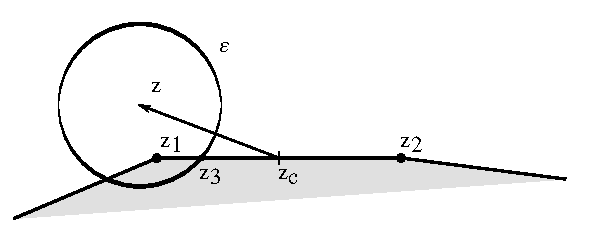
\includegraphics{ConvInfluence.pdf}\end{center}

Если один из концов отрезка является ближним, а другой дальним, 
отрезок делится на две части точкой $\br p_3$, для каждой
из которых влияние вычисляется по своей формуле.
В обычном случае, функцию для блихних вихрей удобней записать без использования
комплексных чисел:
$(\br p_c - \br p)(\br p_2 - \br p_1 ) / \varepsilon^2$

%%%%%%%%%%%%%%%%%%%%%%%%%%%%%%%%%%%%%%%%%%%%%%%%%%%%%%%%%%%%%%%%%%%%%%%%%%%%%%%%
\section{Результаты}
\subsection{Давление}
Давление в точке вычисляется по формуле:
\begin{multline*}
\frac{C_p}{2} = p(\br r) - p_\infty = \frac{1}{2} \left( V^2_\infty - V^2(\br r) \right) 
+\sum\limits_\text{old}{\br u_i \cdot \br V_i} + \\
\
+\frac{1}{\Delta t}\sum\limits_\text{new-old}
{\left\lbrace\left( \br r_{k+1} - \br r_k \right)\left( \br e_z \times \br K(\br r, \br r_k) \right)
\sum_{i=1}^k{\Delta\gamma_i}\right\rbrace} - \\
\
- \frac{1}{\Delta t}\sum\limits_\text{new-old}
{\left\lbrace\left( \br r_{k+1} - \br r_k \right)
\br K(\br r, \br r_k) \sum_{i=1}^k{\Delta q_i}\right\rbrace}
\end{multline*}

Обозначения банальные: $\br r$ --- точка, в которой считаем всё всё всё,
$p$ --- давление.

Первая сумма считается по всем старым (в самом начале шага) элементам ---
свободным вихрям, присоединенным вихрям и источникам. Здесь
$\br u_i$ --- скорость вихря,
$\br V_i$ --- скорость, индуцированная им в точке $\br r$.

Вторая и третья сумма берется по измененным этлементам: по свеже 
вычисленным неизвестным вихрям, и по изменениям присоединенных вихрей, источников.
Внутреннее суммирование ведется вдоль контура. Сумма представляет собой циркуляцию,
народившуюся на данном отрезке за данный шаг. Выбор начала отсчета роли не играет.
$\Delta \gamma_i$ --- инзменение циркуляции в данной точке,
$\Delta q_i$ --- аналогично для интенсивности.

%%%%%%%%%%%%%%%%%%%%%%%%%%%%%%%%%%%%%%%%%%%%%%%%%%%%%%%%%%%%%%%%%%%%%%%%%%%%%%%%
\subsection{Касательное напряжение и сила трения}

В физике есть такая величина, как касательное напряжение (shear stress) $\tau_w = \mu \left. \dfrac{\partial u}{\partial y} \right|_{y=0}$. Вычисляется оно из диффузионной скорости отталкивания от стенки, но с другими порядками суммирования. $ \tau_w = \sum_i {W_d \gamma_i}$. $i$ --- индекс вихря; $k$ --- индекс отрезка. Для простоты используется тот факт, что вблизи стенки $I_0 \approx \pi\varepsilon^2$ и целиком формула выглядит, как

$$ \tau_{wk} = \dfrac{1}{\Reyn}\dfrac{1}{\pi\varepsilon^2} \sum\limits_i dS_k\cdot \gamma_i e^{-\lvert\rho_i\rvert/\varepsilon}$$

Что бы получить конечную силу, эту штуку надо проинтегрировать по поверхности. Это не сложно:

$$ \br F_\tau = \sum_k {\tau_{wk} (\br p_{k+1} - \br p_k) } $$

%%%%%%%%%%%%%%%%%%%%%%%%%%%%%%%%%%%%%%%%%%%%%%%%%%%%%%%%%%%%%%%%%%%%%%%%%%%%%%%%
\subsection{Температура в пространстве}
Каждый тепловой домен представляет собой область конечного размера, интенсивность которой выражается как $q_i = T \cdot dS$. Что бы построить поле температур, и что бы оно было достаточно гладким, мы делаем предположение, что форма каждого теплового домена --- ''Гауссова шапочка``. Отсюда и из условия нормировки получаем
$$T(\rho_i) = \dfrac{q_i}{\pi \varepsilon^2} e^{-\lvert \rho_i \rvert / \varepsilon^2}$$

%%%%%%%%%%%%%%%%%%%%%%%%%%%%%%%%%%%%%%%%%%%%%%%%%%%%%%%%%%%%%%%%%%%%%%%%%%%%%%%%
\subsection{Число Нуссельта}

Локальный: Суммирование ведется по частицам, рожденным и умершим на данном отрезке.
$$\Nuss_\text{loc} = \dfrac{\Reyn \cdot \Pran}{\Delta t \Delta l \Delta T} \sum q_i$$
Средний: Суммирование по всем отрезкам. Для каждого тела свой.
$$\Nuss_\text{avg} = \dfrac{\sum (\Delta l_i \cdot \Nuss_\text{loc})}{\sum \Delta l_i}$$
Интегральный:
$$\Nuss_\text{int} = \sum ( \Delta l_i \cdot \Nuss_\text{loc})$$


%%%%%%%%%%%%%%%%%%%%%%%%%%%%%%%%%%%%%%%%%%%%%%%%%%%%%%%%%%%%%%%%%%%%%%%%%%%%%%%%
\newpage
\section{Diffusive}
\subsection{Vortex diffusive}

$\br r$ - координаты текущего вихря (для которого вычисляем скорость) \\
$\br V_d$ - диффузионная скорость текущего вихря, индуцированная другими вихрями \\
$\varepsilon$ - расстояние от текущего вихря до 2го ближайшего \\
$\br r_j, \gamma_j$ - координата j-го вихря и его циркуляция \\
$\br\rho_j = \br r - \br r_j$ - и так понятно \\

\begin{equation*}
\br I_2 = \dfrac{1}{\varepsilon}
\sum\limits_j (\br\rho_j / \lvert\rho_j\rvert)\cdot\gamma_j e^{-\lvert\rho_j\rvert/\varepsilon},
%\end{equation*}
%\begin{equation*}
I_1 = {\sum\limits_j \gamma_j e^{-\lvert\rho_j\rvert/\varepsilon}},
%\end{equation*}
%\begin{equation*}
\br V_d = \dfrac{1}{\Reyn} \dfrac{\br I_2}{I_1}
\end{equation*}

\begin{center}\setlength\fboxsep{0pt}
\setlength\fboxrule{0.5pt}
\fbox{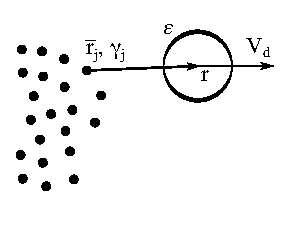
\includegraphics{VortexDiff.pdf}}
\end{center}

%%%%%%%%%%%%%%%%%%%%%%%%%%%%%%%%%%%%%%%%%%%%%%%%%%%%%%%%%%%%%%%%%%%%%%%%%%%%%%%%
\subsection{Body diffusive}

$\br r$ - координаты текущего вихря (для которого вычисляем скорость) \\
$\br W_d$ - диффузионная скорость текущего вихря, индуцированная стенкой \\
$\br p_k$ - k-я вершина тела \\
$\br r_k = \frac{1}{2}(\br p_k + \br p_{k+1})$ - центр k-го отрезка тела \\
$d \br S_k = \br n \cdot\lvert\br p_{k+1} - \br p_k \rvert$ - нормаль к k-му отрезку, с длиной, равной длине отрезка (направление --- из тела в жидкость) \\
$\br{\rho}_k = \br r - \br r_k$ - и так понятно \\

\begin{equation*}
\br I_3 = {\sum\limits_k d\br S_k\cdot e^{-\lvert\rho_k\rvert/\varepsilon}},
%\end{equation*}
%\begin{equation*}
I_0 = {\varepsilon^2\sum\limits_k \dfrac{\lvert\rho_k\rvert /\varepsilon +1}{\rho_k^2}
\cdot(\br\rho_k \cdot d\br S_k)\cdot e^{-\lvert\rho_k\rvert/\varepsilon}},
%\end{equation*}
%\begin{equation*}
\br W_d = \dfrac{1}{\Reyn} \dfrac{\br I_3}{2\pi\varepsilon^2 - I_0}
\end{equation*}

\begin{center}\setlength\fboxsep{0pt}
\setlength\fboxrule{0.5pt}
\fbox{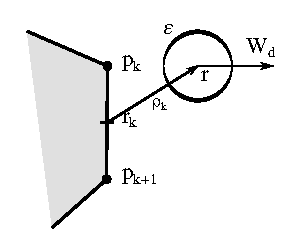
\includegraphics{BodyDiff.pdf}}
\end{center}

%%%%%%%%%%%%%%%%%%%%%%%%%%%%%%%%%%%%%%%%%%%%%%%%%%%%%%%%%%%%%%%%%%%%%%%%%%%%%%%%
\subsection{Heat diffusive}

\begin{equation*}
{\br V_d}_\text{heat} = \frac {1}{\Pran}\frac{1}{\Reyn} \cdot\frac{\br I_2 + \br I_3}{I_1 - I_0}
\end{equation*}

%%%%%%%%%%%%%%%%%%%%%%%%%%%%%%%%%%%%%%%%%%%%%%%%%%%%%%%%%%%%%%%%%%%%%%%%%%%%%%%%
\subsection{Ограничения $\br V_d$ и $\varepsilon$}
В новой версии все идиотизмы исправлены, и ограничение сделано максимально понятным: $I_0$ и $\gamma_i$ должны быть одного знака, и $\lvert I_0 \rvert > 0.1 \lvert\gamma_i\rvert$. 
Для $\varepsilon$ вводится ограничение снизу $\varepsilon > \langle dS_k \rangle$

%%%%%%%%%%%%%%%%%%%%%%%%%%%%%%%%%%%%%%%%%%%%%%%%%%%%%%%%%%%%%%%%%%%%%%%%%%%%%%%%
\newpage
\section{FlowMove}
\subsection{Схема Эйлера (классика)}
\begin{equation*}\begin{split}
&\dot{\br r} = \br V (\br r, t) \\
\Rightarrow~&\br r_{i+1} = \br r_i + \br V(\br r_i, t_i) \cdot \Delta t
\end{split}\end{equation*}

\subsection{Схема Эйлера с пересчетом}
\begin{equation*}\begin{split}
&\dot{\br r} = \br V (\br r, t) \\
\Rightarrow~&\tilde{\br r}_{i+1} = \br r_i + \br V(\br r_i, t_i) \cdot \Delta t \\
\Rightarrow~&\br r_{i+1} = \br r_i + 
\frac{\br V(\br r_i, t_i) + \br V( \tilde{\br r}_{i+1}, t_{i+1})}{2}\cdot \Delta t \\
\end{split}\end{equation*}
А что бы не хранить 2 скорости (или старые координаты) для
каждой частицы, да и вообще упростить работу с модулем,
последюю формулу перепишем в виде
\begin{equation*}
\Rightarrow~\br r_{i+1} = \tilde{\br r}_{i+1} + 
\left( -\br V(\br r_i, t_i) + \br V( \tilde{\br r}_{i+1}, t_{i+1}) \right)\cdot \frac{\Delta t}{2} \\
\end{equation*}

\subsection{Последовательность действий}
\begin{packed_enum}
\item ГУ не выполнены\\
\item Строим дерево
\item Берем скорости набегающего потока итд, заполняем СЛАУ
\item Решаем СЛАУ
\item Удаляем дерево\\
\item Сохраняемся: вихри, тела
\item Спускаем вихри, чернила, тепло\\
\item Строим дерево
\item Считаем эпсилоны, объединяем вихри
\item Считаем скорости: Convective, Diffusive, Boundary; скорости чернил, тепла
\subitem Опционально: двигаем на пол шага, заменяем скорости на отрицательные.
\subitem Опционально: считаем вторую половину скоростей.
\item Двигаем вихри, тела, стриклайны; удаляем проникшие внутрь.
\item Печатаем файл stepdata
\item $t += \Delta t$
\end{packed_enum}

%%%%%%%%%%%%%%%%%%%%%%%%%%%%%%%%%%%%%%%%%%%%%%%%%%%%%%%%%%%%%%%%%%%%%%%%%%%%%%%%
\newpage
\section{Устойчивость и выбор параметров расчета}
Согласно статье в ЖВМ, параметры расчета выбираются исходя из
соображений устойчивости. Параметрами, которые мы можем менять, являются:
$N$ --- число отрезков разбиения контура;\\
$\varepsilon_{min}$ --- ограничение на эпсилон из диффузии;\\
$\Delta t$ --- шаг по времени;\\
$r_d$ --- радиус дискретности, он же эпсилон в конвективной скорости.\\

Дополнительные обозначения:\\
$\Delta l_i$ --- длина i-го отрезка на теле, соответственно \\
$\langle\Delta l \rangle=\dfrac{1}{N} \sum\limits_{i=0}^{N} \Delta l_i$ ---
средняя длина отрезков.\\
$N$ обычно выбирается на глаз.\\
$\varepsilon_{min}=0.6\cdot\langle\Delta l \rangle$ --- 
определено в модуле diffmergefast\\
$\Delta t = \Reyn \varepsilon_{min}^2 < 2 \Reyn \varepsilon^2$\\
$r_d = ?$ --- а этот вопрос остается открытым \\

\subsection{Схемная вязкость}
\begin{equation*}
\nu_\text{сх}^I = 0.018 \cdot \Omega_0^2 r_*^2 \Delta t
\end{equation*}
\begin{equation*}
\nu_\text{сх}^{II} = 5\cdot10^{-4} \cdot \dfrac{\gamma_*^2 a}{r_d^3} \cdot \Delta t
\end{equation*}

Обозначения:\\
$r_*$ --- характерный размер вихря (диаметр)\\
$\Omega_0 = \dfrac{\sum\gamma_i}{\pi r_*^2}$ --- характерная завихренность\\
$\gamma_* = \langle \gamma_i \rangle$ --- средняя циркуляция доменов\\
$a = \sqrt{\pi r_*^2 / N} $ --- характерное расстояние между доменами\\
$r_d$ --- радиус дискретности\\

%%%%%%%%%%%%%%%%%%%%%%%%%%%%%%%%%%%%%%%%%%%%%%%%%%%%%%%%%%%%%%%%%%%%%%%%%%%%%%%%
\newpage
\section{Сохранение результатов}

\subsection{Бинарники с каждого шага}
Первые 1024 байта --- закладки. Каждая закладка 16 байт. 8 байт --- название (восемь букв, и еще 8 --- указатель (номер байта в файле).\\
``Header  '' --- Общая инфа о режиме, задаваемая из мейн файла. И после этого последовотельно по 8 байт $\Delta t$, $1/\nu$, $V_{x\infty}$, $V_{y\infty}$, real time (timet), T.\\
``Vortexes'', ``Heat    '', ``StrkSrc '', ``Streak  '', ``Body    '' --- различные списки. У каждого списка первые 8 байт занимает количество элементов $N$. Оставшиеся $8\cdot 3 \cdot N$ байт уходят на массив троек ($r_x$, $r_y$, g). У списка ``Body    '' последней тройкой хранится (RotAxis.rx, RotAxis.ry, $\omega$)


\subsection{Профили трения, давления, и теплоотдачи}
Первые $2 \cdot 4$байта --- TValues, N.\\
TValues --- это enum. $C_p=1$, $Fr=2$, $Nu=4$.\\
N --- число отрезков на всех телах.\\
На каждом временном шаге сохраняется сначала текущее время (4 байта). Далее идут группы по 3--5 floatов: ($r_x$, $r_y$, [$C_p$], [$Fr$], [$Nu$])

\end{document}
